%%%% Paramétrage du TD %%%%
\def\xxnumchapitre{Chapitre 0 \vspace{.2cm}}
\def\xxchapitre{\hspace{.12cm} Prise en main de Python}

\def\xxcompetences{%
\textsl{%
\textbf{Savoirs et compétences :}\\
\vspace{-.4cm}
\begin{itemize}[label=\ding{112},font=\color{bleuxp}] 
\item .
%\item \textit{Mod3.C2 : } pôles dominants et réduction de l’ordre du modèle : principe, justification
%\item \textit{Res2.C4 : } stabilité des SLCI : définition entrée bornée -- sortie bornée (EB -- SB)	
%\item \textit{Res2.C5 : } stabilité des SLCI : équation caractéristique	
%\item \textit{Res2.C6 : } stabilité des SLCI : position des pôles dans le plan complexe
%\item \textit{Res2.C7 : } stabilité des SLCI : marges de stabilité (de gain et de phase)
\end{itemize}
}}


\def\xxfigures{
%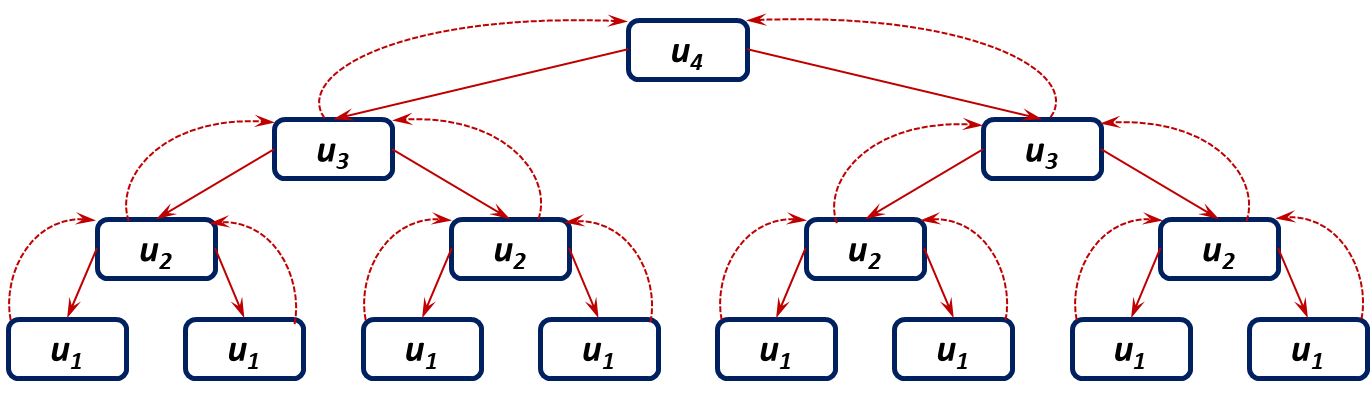
\includegraphics[width=3cm]{fig_01}\\
%\textit{}
}%figues de la page de garde

\def\xxtitreexo{Applications -- Bases}
\def\xxsourceexo{}
\def\xxactivite{{ Application 01} \ifprof  -- Corrigé \else \fi}

%\iflivret
\input{\repRel/Style/pagegarde_TD}
%\else
%\pagestyle{empty}


%%%%%%%% PAGE DE GARDE COURS
\ifcours
\begin{tikzpicture}[remember picture,overlay]
\node at (current page.north west)
{\begin{tikzpicture}[remember picture,overlay]
\node[anchor=north west,inner sep=0pt] at (0,0) {\includegraphics[width=\paperwidth]{\thechapterimage}};
\draw[anchor=west] (-2cm,-8cm) node [line width=2pt,rounded corners=15pt,draw=ocre,fill=white,fill opacity=0.6,inner sep=40pt]{\strut\makebox[22cm]{}};
\draw[anchor=west] (1cm,-8cm) node {\huge\sffamily\bfseries\color{black} %
\begin{minipage}{1cm}
\rotatebox{90}{\LARGE\sffamily\textsc{\color{ocre}\textbf{\xxnumpartie}}}
\end{minipage} \hfill
\begin{minipage}[c]{14cm}
\begin{titrepartie}
\begin{flushright}
\renewcommand{\baselinestretch}{1.1} 
\Large\sffamily\textsc{\textbf{\xxpartie}}
\renewcommand{\baselinestretch}{1} 
\end{flushright}
\end{titrepartie}
\end{minipage} \hfill
\begin{minipage}[c]{3.5cm}
{\large\sffamily\textsc{\textbf{\color{ocre} \discipline}}}
\end{minipage} 
 };
\end{tikzpicture}};
\end{tikzpicture}


\begin{tikzpicture}[overlay]
\node[shape=rectangle, 
      rounded corners = .25 cm,
	  draw= ocre,
	  line width=2pt, 
	  fill = ocre!10,
	  minimum width  = 2.5cm,
	  minimum height = 3cm,] at (18cm,0) {};
\node at (17.7cm,0) {\rotatebox{90}{\textbf{\Large\color{ocre}{\classe}}}};
%{};
\end{tikzpicture}

\vspace{3.5cm}

\begin{tikzpicture}[remember picture,overlay]
\draw[anchor=west] (-2cm,-6cm) node {\huge\sffamily\bfseries\color{black} %
\begin{minipage}{2cm}
\begin{center}
\LARGE\sffamily\textsc{\color{ocre}\textbf{\xxactivite}}
\end{center}
\end{minipage} \hfill
\begin{minipage}[c]{15cm}
\begin{titrechapitre}
\renewcommand{\baselinestretch}{1.1} 
\Large\sffamily\textsc{\textbf{\xxnumchapitre}}

\Large\sffamily\textsc{\textbf{\xxchapitre}}
\vspace{.5cm}

\renewcommand{\baselinestretch}{1} 
\normalsize\normalfont
\xxcompetences
\end{titrechapitre}
\end{minipage}  };
\end{tikzpicture}
\vfill

\begin{flushright}
\begin{minipage}[c]{.3\linewidth}
\begin{center}
\xxfigures
\end{center}
\end{minipage}\hfill
\begin{minipage}[c]{.6\linewidth}
\startcontents
\printcontents{}{1}{}
\end{minipage}
\end{flushright}

\begin{tikzpicture}[remember picture,overlay]
\draw[anchor=west] (4.5cm,-.7cm) node {
\begin{minipage}[c]{.2\linewidth}
\begin{flushright}

\includegraphics[width=2cm]{png/logoCC}
\end{flushright}
\end{minipage}
\begin{minipage}[c]{.2\linewidth}
\textsl{\xxauteur} \\
\textsl{\classe}
\end{minipage}
 };
\end{tikzpicture}
\newpage
\pagestyle{fancy}

\newpage
\pagestyle{fancy}

\else
\fi


%%%%%%%% PAGE DE GARDE TD
\iftd
%\begin{tikzpicture}[remember picture,overlay]
%\node at (current page.north west)
%{\begin{tikzpicture}[remember picture,overlay]
%\draw[anchor=west] (-2cm,-3.25cm) node [line width=2pt,rounded corners=15pt,draw=ocre,fill=white,fill opacity=0.6,inner sep=40pt]{\strut\makebox[22cm]{}};
%\draw[anchor=west] (1cm,-3.25cm) node {\huge\sffamily\bfseries\color{black} %
%\begin{minipage}{1cm}
%\rotatebox{90}{\LARGE\sffamily\textsc{\color{ocre}\textbf{\xxnumpartie}}}
%\end{minipage} \hfill
%\begin{minipage}[c]{13.5cm}
%\begin{titrepartie}
%\begin{flushright}
%\renewcommand{\baselinestretch}{1.1} 
%\Large\sffamily\textsc{\textbf{\xxpartie}}
%\renewcommand{\baselinestretch}{1} 
%\end{flushright}
%\end{titrepartie}
%\end{minipage} \hfill
%\begin{minipage}[c]{3.5cm}
%{\large\sffamily\textsc{\textbf{\color{ocre} \discipline}}}
%\end{minipage} 
% };
%\end{tikzpicture}};
%\end{tikzpicture}

%%%%%%%%%% PAGE DE GARDE TD %%%%%%%%%%%%%%%
%\begin{tikzpicture}[overlay]
%\node[shape=rectangle, 
%      rounded corners = .25 cm,
%	  draw= ocre,
%	  line width=2pt, 
%	  fill = ocre!10,
%	  minimum width  = 2.5cm,
%	  minimum height = 2.5cm,] at (18.5cm,0) {};
%\node at (17.7cm,0) {\rotatebox{90}{\textbf{\Large\color{ocre}{\classe}}}};
%%{};
%\end{tikzpicture}

% PARTIE ET CHAPITRE
%\begin{tikzpicture}[remember picture,overlay]
%\draw[anchor=west] (-1cm,-2.1cm) node {\large\sffamily\bfseries\color{black} %
%\begin{minipage}[c]{15cm}
%\begin{flushleft}
%\xxnumchapitre \\
%\xxchapitre
%\end{flushleft}
%\end{minipage}  };
%\end{tikzpicture}

% Bandeau titre exo
\begin{tikzpicture}[remember picture,overlay]
\draw[anchor=west] (-2cm,-4cm) node {\huge\sffamily\bfseries\color{black} %
\begin{minipage}{5cm}
\begin{center}
\LARGE\sffamily\color{ocre}\textbf{\textsc{\xxactivite}}

\begin{center}
\xxfigures
\end{center}

\end{center}
\end{minipage} \hfill
\begin{minipage}[c]{12cm}
\begin{titrechapitre}
\renewcommand{\baselinestretch}{1.1} 
\large\sffamily\textbf{\textsc{\xxtitreexo}}

\small\sffamily{\textbf{\textit{\color{black!70}\xxsourceexo}}}
\vspace{.5cm}

\renewcommand{\baselinestretch}{1} 
\normalsize\normalfont
\xxcompetences
\end{titrechapitre}
\end{minipage}  };
\end{tikzpicture}
\else
\fi


%%%%%%%% PAGE DE GARDE FICHE
\iffiche
\begin{tikzpicture}[remember picture,overlay]
\node at (current page.north west)
{\begin{tikzpicture}[remember picture,overlay]
\draw[anchor=west] (-2cm,-3.25cm) node [line width=2pt,rounded corners=15pt,draw=ocre,fill=white,fill opacity=0.6,inner sep=40pt]{\strut\makebox[22cm]{}};
\draw[anchor=west] (1cm,-3.25cm) node {\huge\sffamily\bfseries\color{black} %
\begin{minipage}{1cm}
\rotatebox{90}{\LARGE\sffamily\textsc{\color{ocre}\textbf{\xxnumpartie}}}
\end{minipage} \hfill
\begin{minipage}[c]{14cm}
\begin{titrepartie}
\begin{flushright}
\renewcommand{\baselinestretch}{1.1} 
\large\sffamily\textsc{\textbf{\xxpartie} \\} 

\vspace{.2cm}

\normalsize\sffamily\textsc{\textbf{\xxnumchapitre -- \xxchapitre}}
\renewcommand{\baselinestretch}{1} 
\end{flushright}
\end{titrepartie}
\end{minipage} \hfill
\begin{minipage}[c]{3.5cm}
{\large\sffamily\textsc{\textbf{\color{ocre} \discipline}}}
\end{minipage} 
 };
\end{tikzpicture}};
\end{tikzpicture}


\begin{tikzpicture}[overlay]
\node[shape=rectangle, 
      rounded corners = .25 cm,
	  draw= ocre,
	  line width=2pt, 
	  fill = ocre!10,
	  minimum width  = 2.5cm,
	  minimum height = 2.5cm,] at (18.5cm,0.5cm) {};
%	  minimum height = 2.5cm,] at (18.5cm,0cm) {};
\node at (17.7cm,0.5) {\rotatebox{90}{\textsf{\textbf{\large\color{ocre}{\classe}}}}};
%{};
\end{tikzpicture}

\else
\fi



%\fi

\setlength{\columnseprule}{.1pt}

\pagestyle{fancy}
\thispagestyle{plain}


\vspace{4.5cm}

\def\columnseprulecolor{\color{bleuxp}}
\setlength{\columnseprule}{0.4pt} 

%%%%%%%%%%%%%%%%%%%%%%%




\ifprof
\vspace{1cm}
\else
\begin{multicols}{2}
\fi




\subsection*{Découverte de quelques types dans l'interpréteur}
Lancer PYZO.\\
Une fenêtre s'ouvre sur votre écran partagée en 3 zones, il est nécessaire d'ouvrir le shell en choisissant la version de python, alors quelques lignes de message introductif s'inscrivent. C'est l'\textbf{interpréteur} de Python, qu'on appelle aussi le \textbf{shell}.\\
Les symboles \texttt{{>}{>}{>}} invitent à taper quelque chose (invite de commande). \\

\textbf{Fonctionnement} : tapez une \emph{instruction}, par exemple $1+1$,  et tapez "Entrée" : 

\begin{lstlisting}
 >>> 1 + 1
        2
\end{lstlisting}

\subsection*{Différents types de nombres}
Le shell de Python peut s'utiliser comme une calculatrice pour manipuler des nombres. Selon la nature (entiers, réels, complexes) des nombres que l'on souhaite manipuler, il y aura différents \emph{types} sous python pour les représenter.\\

Ci-dessus, on a manipulé \texttt{1} qui est de type \texttt{integer} (\emph{entier} en anglais).\\
On manipule aussi les "nombres à virgule", dits nombres \emph{flottants}, dont le type s'appelle \texttt{float} en python : 
\begin{lstlisting}
>>> 3.1 + 10.09
        13.19
>>> type(2.7)
        <type 'float'>
\end{lstlisting}

\begin{warn}Bien remarquer que l'on utilise la convention anglosaxonne : un point et non une virgule.\end{warn}

\exer{}~\\

\question{ Taper les deux instructions suivantes : \texttt{3} , \texttt{3.0} puis \texttt{'3'} puis demander le type de ces données. Commenter}

\ifprof
\begin{corrige}
Python n'affiche pas le même résultat ; ce sont bien deux objets différents car de type différent.
 \end{corrige}
 \else
 \fi
 
 
\question{Taper les trois instructions suivantes : \texttt{3.}, \texttt{0.1} puis \texttt{.1}. Commenter.}
\ifprof
\begin{corrige}{On peut parfois se passer du 0 dans l'écriture à virgule, lorsque c'est le seul chiffre à gauche ou à droite du point.}
\end{corrige}
\else\fi

%
%\begin{donnees}
%Ce qu'il faut retenir: \\
%{}
%{}
%\end{donnees}

\exer{}\\
\question{Testez les opérateurs suivants avec des entiers et/ou des flottants :}
 \begin{center}
 \texttt{ -\quad  * \quad  / \quad // \quad \% \quad \^{} \quad **}
\end{center}

\question{Que dire du résultat et du type du résultat pour les opérateurs \texttt{/}, \texttt{//} et \texttt{\%}, par exemple comment relier les résultats obtenus de ces deux opérations: 9\texttt{//}2 et 9\texttt{\%}2 ?
L'opérateur \texttt{\^{}} renvoie-t-il le résultat attendu ? Que ce passe-t-il en cas d'opération entre un entier et un flottant ?}
\ifprof
\begin{corrige}
{Les opérateurs +, - * marchent comme attendu, mais on remarque tout de suite qu'une opération entre un flottant et un entier est toujours un flottant.\\}
{/ permet la division et renvoie toujours un flottant, même pour 4/2 par exemple.\\ // et \% donnent le quotient et le reste dans la division euclidienne de deux entiers, ce sont des entiers : (a//b donne q et a\% b donne r où q et r sont les entiers tels que a=bq+r et 0<=0<b.)\\}
{\^{} ne donne pas du tout la puissance (c'est le "ou exclusif bit à bit), c'est ** qu'il faut utiliser.}

\end{corrige}
\else
\fi
%%\begin{donnees}
%\texttt{Ce qu'il faut retenir :}\\
%\texttt{+;-;*;/:}\\
%\texttt{//;\% :}\\
%\texttt{\^{} :}\\
%\texttt{** :}\\
%%\end{donnees}

Les fonctions \texttt{float} et \texttt{int} permettent d'obtenir une donnée du type voulu. Taper les instructions suivantes, où l'on voit des premiers exemples d'\emph{affectations}, ici des \emph{variables} \texttt{x} et \texttt{y} : 
\ifprof
\begin{lstlisting}
>>> x = 42
>>> x 
................. \textit{à compléter !}\cache{42}
>>> float(x)
................. \cache{42.0} 
>>> y = -3.67\\
>>> y \\
.................\cache{-3.67} 
>>> int(y)\\
................. \cache{-3}
\end{lstlisting}
\else
\begin{lstlisting}
>>> x = 42
>>> x 
................. \textit{à compléter !}
>>> float(x)
................. 
>>> y = -3.67\\
>>> y \\
.................
>>> int(y)\\
.................
\end{lstlisting}
\fi

\begin{warn}
 \texttt{int} appliqué à un flottant ne fait pas un arrondi, ni ne calcule la partie entière : cela donne juste l'entier qui apparaît dans l'écriture décimale du flottant.\
 \end{warn}




\subsection*{Les booléens}

Une variable de type booléen ne peut prendre que deux valeurs: \texttt{True} ou \texttt{False}. Il s'agit souvent de propositions logiques plus ou moins longues que python peut évaluer. 
 Quelques exemples : 
\begin{lstlisting} 
>>> 1 > 0
        True
>>> a = (1 > 3)
>>> a
        False 
>>> type(a)
        <type 'bool'>
>>> x = 3.14
>>> y = 3.1
>>> x == y 
        False
\end{lstlisting}
%\newpage

Les opérateurs de comparaison disponibles sont :

%\begin{donnees}
\begin{center}
\begin{tabular}{>{\ttfamily}cc}
\hline
x == y&$x$ est égal à $y$\\
x != y & $x$ est différent de $y$\\
x > y & $x$ est strictement supérieur à $y$\\
x < y & $x$ est strictement inférieur à $y$\\
x >= y& $x$ est supérieur ou égal à $y$\\
x <= y& $x$ est inférieur ou égal à $y$\\
\hline
\end{tabular}
\end{center}

Bien noter la différence entre \texttt{=} (pour affecter une variable se trouvant à gauche du signe) et \texttt{==} (pour définir une égalité qui sera un booléen).\\
Pour combiner des variables booléennes, on dispose de trois opérateurs logiques : \texttt{ not}, \texttt{and}, \texttt{or}. 
%\end{donnees}


\exer{}

\question{Créer une variable \texttt{x} égale à l'entier 3, et tester les trois opérateurs logiques ci-dessus sur les expressions \texttt{x  < 4.1} et \texttt{x \% 2 == 0}.}

\question{Mathématiquement, à quoi correspond le booléen \texttt{x \% 2 == 0} ?} 


%On rappelle qu'une proposition  $P\ ou \ Q$ est vraie si et seulement si l'une au moins des propositions est vraie, \textbf{éventuellement les deux}. Ce n'est pas le "ou exclusif" que l'on trouve par exemple  sur les menus de restaurants : "Fromage ou dessert" (on ne peut pas avoir à la fois le fromage et le dessert... avec le "ou logique", c'est tout-à-fait admis.)

\subsection*{Les chaînes de caractères}
Python permet aussi de manipuler du texte. Le type utilisé 
s'appelle une chaîne de caractère : \textit{string} en anglais, abrégé en \texttt{str} en Python. Il suffit de délimiter le texte par des apostrophes (\textit{quote}) ou par des guillemets (\textit{double quote}) :
\begin{lstlisting}
>>> c = 'ptsi'
>>> d = "bonjour à tous"
\end{lstlisting}





On peut avoir accès aux caractères qui composent une chaîne de caractères ; attention, en Python, ils sont numérotés à partir de 0, c'est-à-dire que le premier caractère est d'indice $0$. 


\question{Noter les résultats et commenter.}
\begin{lstlisting}
>>> c[0]
>>> c[2]
>>> c[-1]
>>> c[0] = 'm' 
\end{lstlisting}
%$\dots\dots\dots\dots\dots\dots$\cache{commentaire : premier caractère}\\
%$\dots\dots\dots\dots\dots\dots$\cache{commentaire : dernier caractère}\\
%$\dots\dots\dots\dots\dots\dots$\cache{message d'erreur, commentaire : une chaine n'est pas "mutable"}

%\begin{donnees}
Trois autres choses à retenir sur le type \texttt{string} : 
\begin{itemize}
\item la longueur d'une chaîne de caractères, c'est-à-dire le nombre de caractères qui la composent, s'obtient avec la fonction \texttt{len}.\\ Tester avec \texttt{c} et \texttt{d}.
\item on peut concaténer des chaînes de caractères (c'est-à-dire les "accoler") à l'aide de \texttt{+}.
\item comme pour les fonctions \texttt{int} et \texttt{float}, il existe une fonction \texttt{str} qui permet d'obtenir un objet de type string.\\
\end{itemize}
%\end{donnees}

\question{Créer une chaîne de caractère \texttt{e} obtenue en concaténant \texttt{c} et \texttt{d}.}

\question{Tester les instructions suivantes ; comment modifier \textbf{la dernière} pour qu'il n'y ait pas de message d'erreur ? }
\begin{lstlisting}
>>> numero = 2
>>> f = c + numero
\end{lstlisting}
%\cache{f = c + str(numero)}

\emph{Remarque:} Le fait qu'un même opérateur (ici \texttt{+}) puisse fonctionner différemment en fonction du contexte illustre le mécanisme appelé \emph{surcharge des opérateurs}.\\



\emph{Remarque : Pour ne pas avoir à tout recopier à chaque ligne du shell en cas d'erreur...}\\
Sous PYZO (windows), Avec la flèche $\uparrow$ (éventuellement plusieurs fois successivement), on peut remonter dans l'historique de commandes.\\
Sous IDLE, Se placer sur la ligne à répéter et "entrée".





\ifprof
\else
\end{multicols}
\fi

